\documentclass[11pt, oneside]{article}   	% use "amsart" instead of "article" for AMSLaTeX format
\usepackage{geometry}                		% See geometry.pdf to learn the layout options. There are lots.
\geometry{letterpaper}                   		% ... or a4paper or a5paper or ... 
%\geometry{landscape}                		% Activate for for rotated page geometry
%\usepackage[parfill]{parskip}    		% Activate to begin paragraphs with an empty line rather than an indent
\usepackage{graphicx}				% Use pdf, png, jpg, or eps§ with pdflatex; use eps in DVI mode
								% TeX will automatically convert eps --> pdf in pdflatex		
\usepackage{amssymb}

\title{SE 464 Project Proposal -- Shots Fired}
\author{Sam Maier (scmaier), Addison Keizer (wcakeize), \\Dhruv Lal (d2lal), Shiranka Miskin (samiskin)}
%\date{}							% Activate to display a given date or no date
\let\endtitlepage\relax
\begin{document}
\maketitle
\section{The Project}
%\subsection{}
\indent Our project is a 2-4 player 2D multiplayer platformer shooter game. The multiplayer will be online. The best analogy to describe it is a fusion of Super Smash Bros and Metroid. To build this application we will use Typescript, a modified Javascript. Node.js will be our backend. \\

This project is interesting for both technical and market availability. There is an opening in the market for a well made, free and fun web application that has easy inter-friend multiplayer capability through the internet. There are a ton of games that are very popular multiplayer component   \\

Technology wise this project is even more interesting. The software must be constructed in such a way that the multiplayer appears seamless to the users, which is a significant challenge when done from the beginning and very interesting. Furthermore this gives us the opportunity to learn new a new language in Typescript. This project will also have interesting software architecture because there will need to be a well structured set of software components to represent game objects and the different players and networking tasks. The selection of Node.js as backend means that it will be easier to duplicate game logic between clients and server and we will be able to reuse code. \\

This project makes sense in the chosen environment for a variety of reasons. Our goal for this is to make a fluid and responsive game in on the web to give the users the easiest possible conditions to join into a game with their friends. No install - no setup time. Mobile or desktop both have large mental barriers to entry and our aim is to tear those down. Not to mention that it is completely environment agnostic Mac, PC, Linux - it works for all. In terms of the software directly, this project will give us a chance to learn new technologies all the while working on a challenging problem, the implementation of multiplayer.  \\

\clearpage

\section{Functional Requirements}
\begin{enumerate}
\item Is 2-4 player, each player plays on their own computer. 
\begin{enumerate}
\item Player will be able to control their avatar using keyboard and/or mouse. 
\end{enumerate}
\item Capability for user to join a matched game
\item Capability for user to play with known people in an isolated environment
\item Is a 2D platformer arena style game
\begin{enumerate}
\item 2-4 human players have their own character, and must navigate a small 2d map
\item Numerical based health.
\item A life is lost if you leave the map.
\item Each player has a finite number of lives, set at the beginning of the game
\item Each player has a default weapon with infinite ammo
\end{enumerate}
\item Can handle multiple simultaneous games
\end{enumerate}

\section{User Scenarios}

Consider a user that is with 2 other friends and they are just trying to pass the time or have some fun. They each have their own laptops. Shots Fired is a 2-4 player game and is a game that everyone can play together. This satisfies the need of getting everyone involved in the same activity. To create a game with friends, one person would create a game and choose the option to play with friends. In this case, they will receive a code that their friends can input and use to join the same group. This way, friends can play together and not have to worry about having other people in their game. \\

Each player will control a character on a small 2D map. They will use the mouse and/or keyboard to fire their weapon. If hit, they lose health. When health is 0 they lose. A user would be able to complete a game in under 5 minutes so it is very quick and easy to play anytime. Due to the fact they are playing with friends, there is a bit of a competition between them, however, they are mainly playing for fun to pass the time.  \\



\section{Non Functional Properties} 
\begin{enumerate}
\item Output is rendered without noticeable lag between players if players are on computers with a reasonable internet connection. 
\item Very easy to join a game. Low entry barrier. 
\item Compatible with Chrome 52+.
\end{enumerate}


\clearpage

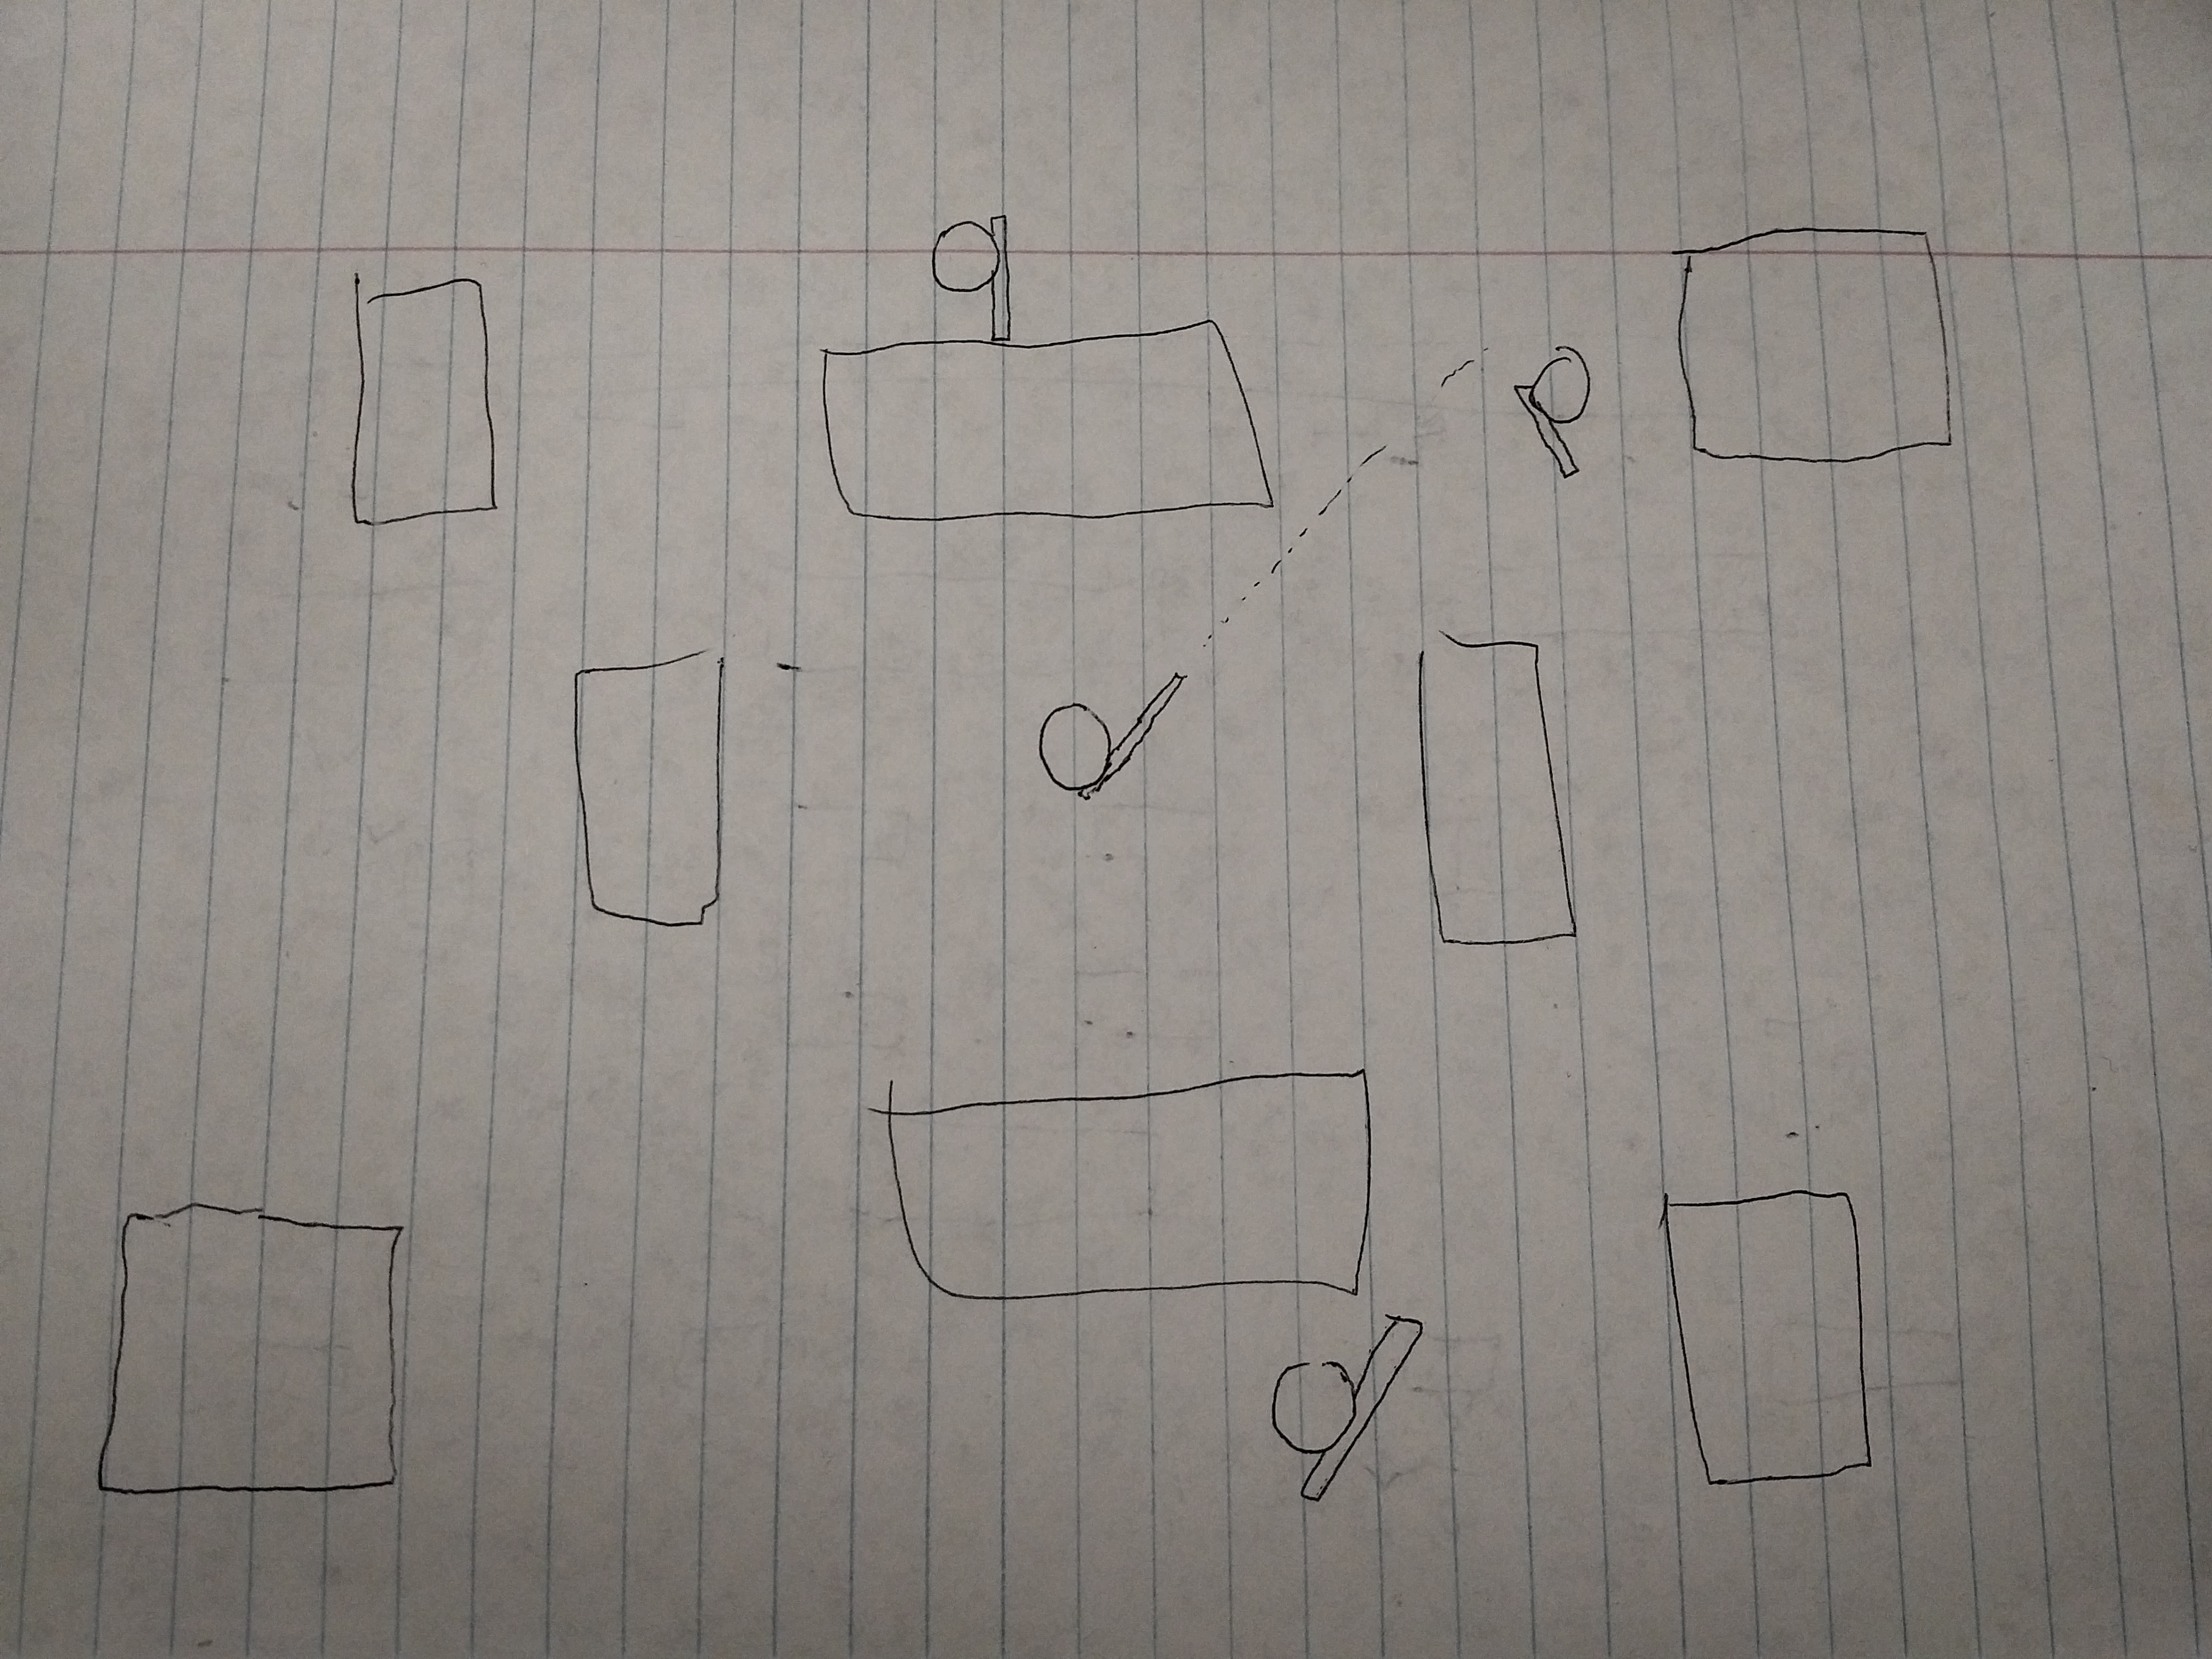
\includegraphics[scale=.09]{mockup.jpg}


\end{document}  